\documentclass[11pt]{article}

\usepackage{amsmath}
\usepackage{graphicx}
\usepackage[margin=2cm]{geometry}

\begin{document}
	La susceptibilidad corresponde con:
	\begin{equation}
	\chi = \dfrac{\partial P}{\partial E} = \dfrac{Z_0}{\beta V^N}\dfrac{\partial^2}{\partial E^2}\left(\dfrac{\sinh(\beta E\mu)}{\beta E\mu}\right)^N
	\end{equation}
	\tiny
	\begin{equation}
	\dfrac{\partial^2}{\partial E^2}\left(\dfrac{\sinh(\beta E\mu)}{\beta E\mu}\right)^N = 	\frac{N \left(\frac{\sinh{\left (E \beta \mu \right )}}{E \beta \mu}\right)^{N}}{E^{2} \left(\cosh{\left (2 E \beta \mu \right )} - 1\right)} \left(E^{2} N \beta^{2} \mu^{2} \cosh{\left (2 E \beta \mu \right )} + E^{2} N \beta^{2} \mu^{2} - 2 E^{2} \beta^{2} \mu^{2} - 2 E N \beta \mu \sinh{\left (2 E \beta \mu \right )} + N \cosh{\left (2 E \beta \mu \right )} - N + \cosh{\left (2 E \beta \mu \right )} - 1\right)
	\end{equation}
	
	\begin{figure}[h]
		\centering
		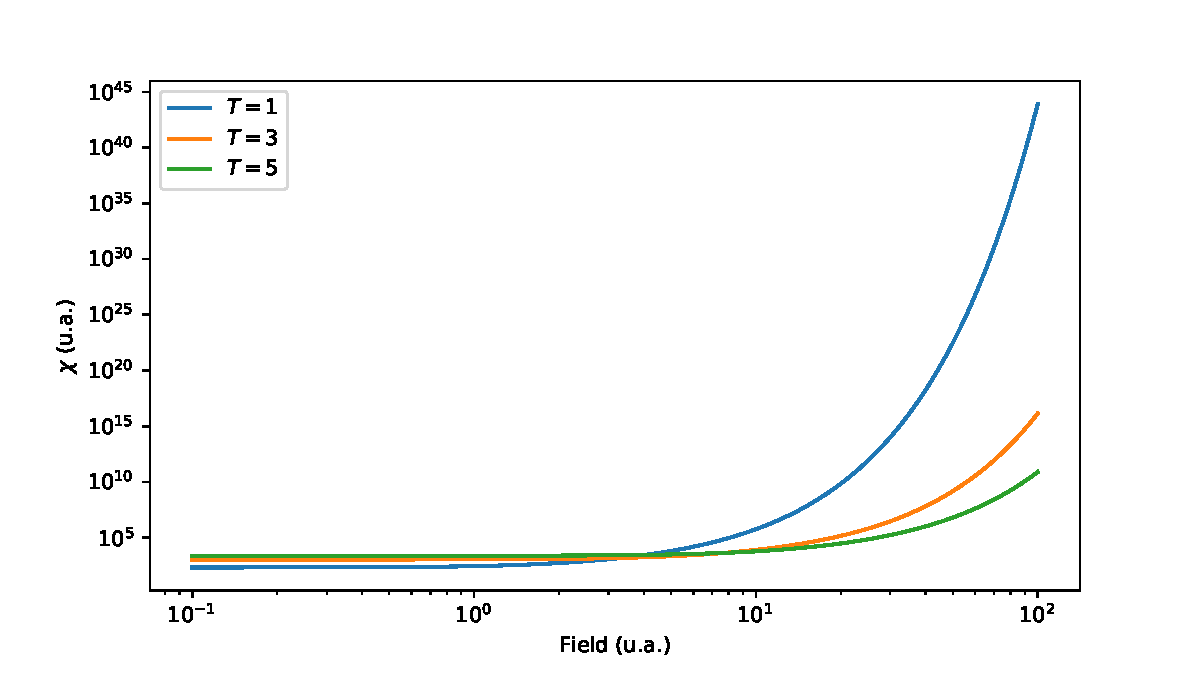
\includegraphics[height=0.3\textheight]{Susceptibility.pdf}
	\end{figure}
	
	\begin{figure}[h]
		\centering
		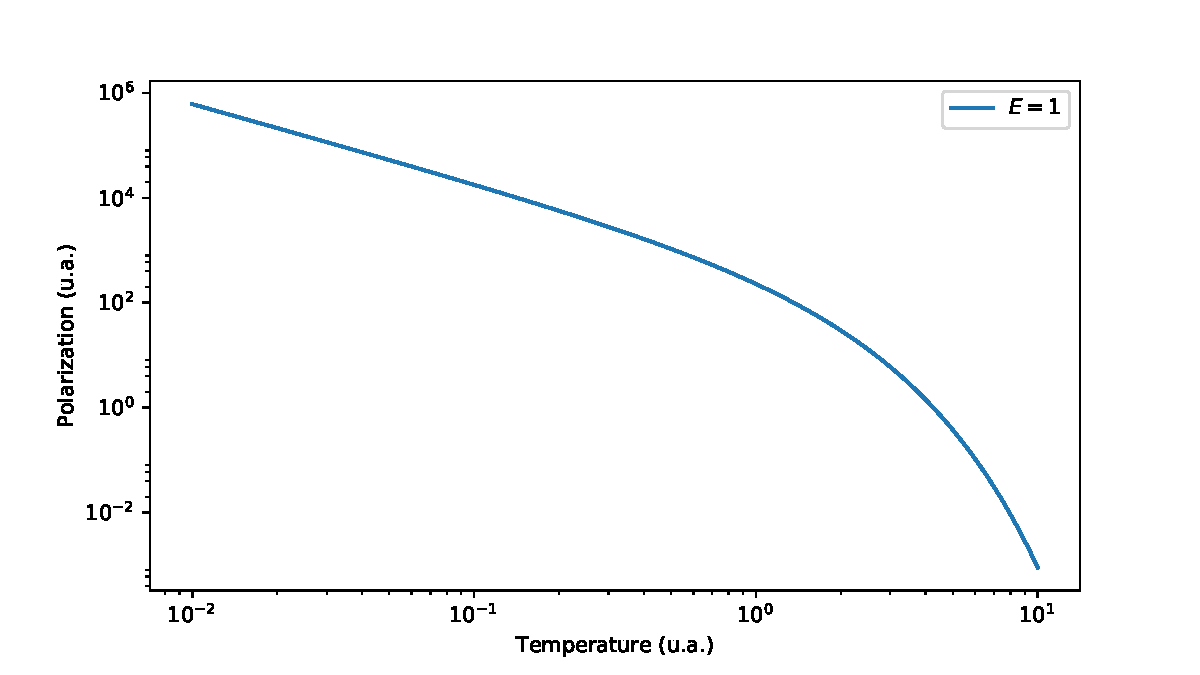
\includegraphics[height=0.3\textheight]{Temperature.pdf}
		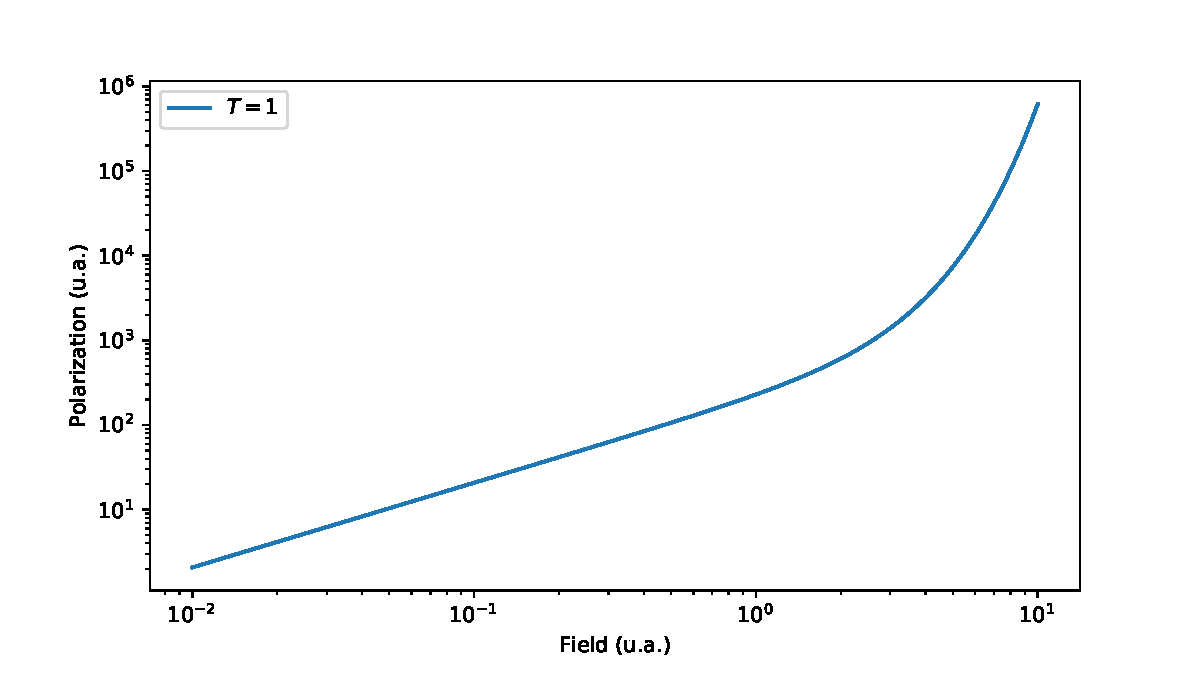
\includegraphics[height=0.3\textheight]{Field.pdf}
		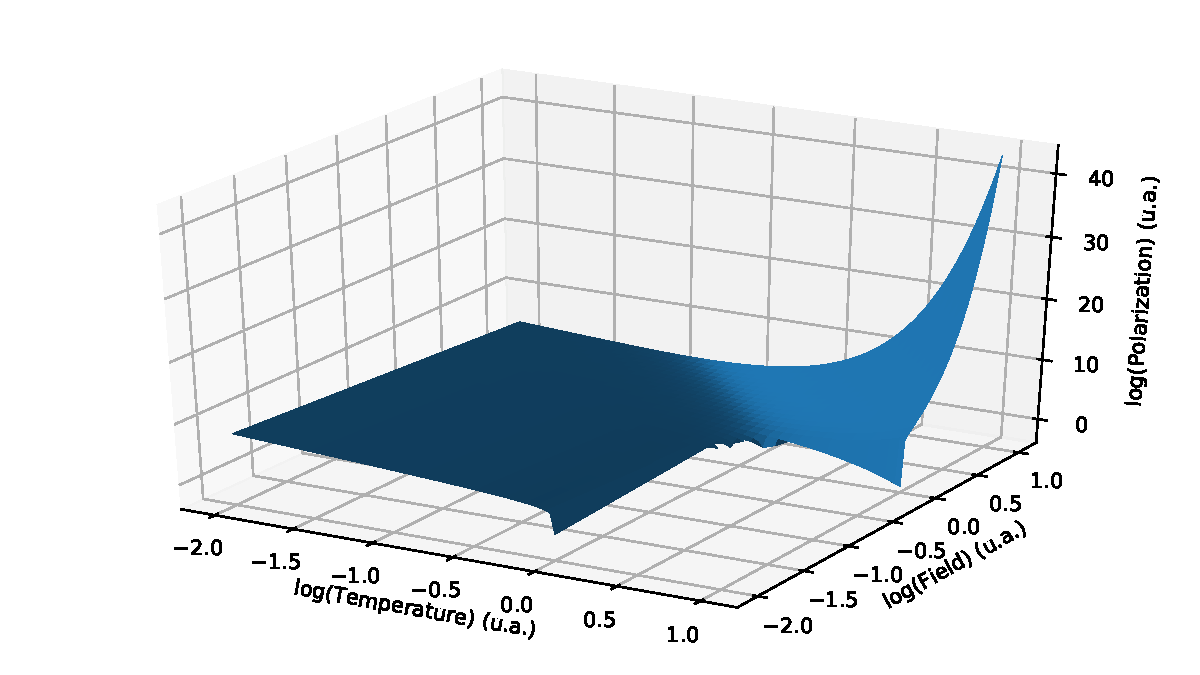
\includegraphics[height=0.3\textheight]{Both.pdf}
	\end{figure}
\end{document}
